
\documentclass[12pt]{article}
%\usepackage[finnish]{babel}
\usepackage[T1]{fontenc}
\usepackage[utf8]{inputenc}
\usepackage{amssymb}
\usepackage{amsmath}
\usepackage{graphicx}
\usepackage{hyperref}
\newcommand{\pat}{\partial}
\newcommand{\be}{\begin{equation}}
\newcommand{\ee}{\end{equation}}
\newcommand{\bea}{\begin{eqnarray}}
\newcommand{\eea}{\end{eqnarray}}
\newcommand{\abf}{{\bf a}}
\newcommand{\Zcal}{{\cal Z}_{12}}
\newcommand{\zcal}{z_{12}}
\newcommand{\Acal}{{\cal A}}
\newcommand{\Fcal}{{\cal F}}
\newcommand{\Ucal}{{\cal U}}
\newcommand{\Vcal}{{\cal V}}
\newcommand{\Ocal}{{\cal O}}
\newcommand{\Rcal}{{\cal R}}
\newcommand{\Scal}{{\cal S}}
\newcommand{\Lcal}{{\cal L}}
\newcommand{\Hcal}{{\cal H}}
\newcommand{\hsf}{{\sf h}}
\newcommand{\half}{\frac{1}{2}}
\newcommand{\Xbar}{\bar{X}}
\newcommand{\xibar}{\bar{\xi }}
\newcommand{\barh}{\bar{h}}
\newcommand{\Ubar}{\bar{\cal U}}
\newcommand{\Vbar}{\bar{\cal V}}
\newcommand{\Fbar}{\bar{F}}
\newcommand{\zbar}{\bar{z}}
\newcommand{\wbar}{\bar{w}}
\newcommand{\zbarhat}{\hat{\bar{z}}}
\newcommand{\wbarhat}{\hat{\bar{w}}}
\newcommand{\wbartilde}{\tilde{\bar{w}}}
\newcommand{\barone}{\bar{1}}
\newcommand{\bartwo}{\bar{2}}
\newcommand{\nbyn}{N \times N}
\newcommand{\repres}{\leftrightarrow}
\newcommand{\Tr}{{\rm Tr}}
\newcommand{\tr}{{\rm tr}}
\newcommand{\ninfty}{N \rightarrow \infty}
\newcommand{\unitk}{{\bf 1}_k}
\newcommand{\unitm}{{\bf 1}}
\newcommand{\zerom}{{\bf 0}}
\newcommand{\unittwo}{{\bf 1}_2}
\newcommand{\holo}{{\cal U}}
%\newcommand{\bra}{\langle}
%\newcommand{\ket}{\rangle}
\newcommand{\muhat}{\hat{\mu}}
\newcommand{\nuhat}{\hat{\nu}}
\newcommand{\rhat}{\hat{r}}
\newcommand{\phat}{\hat{\phi}}
\newcommand{\that}{\hat{t}}
\newcommand{\shat}{\hat{s}}
\newcommand{\zhat}{\hat{z}}
\newcommand{\what}{\hat{w}}
\newcommand{\sgamma}{\sqrt{\gamma}}
\newcommand{\bfE}{{\bf E}}
\newcommand{\bfB}{{\bf B}}
\newcommand{\bfM}{{\bf M}}
\newcommand{\cl} {\cal l}
\newcommand{\ctilde}{\tilde{\chi}}
\newcommand{\ttilde}{\tilde{t}}
\newcommand{\ptilde}{\tilde{\phi}}
\newcommand{\utilde}{\tilde{u}}
\newcommand{\vtilde}{\tilde{v}}
\newcommand{\wtilde}{\tilde{w}}
\newcommand{\ztilde}{\tilde{z}}
\newcommand{\ket}[1]{\vert{#1}\rangle}
\newcommand{\bra}[1]{\langle{#1}\vert}

\usepackage{listings}


\hoffset 0.5cm
\voffset -0.4cm
\evensidemargin -0.2in
\oddsidemargin -0.2in
\topmargin -0.2in
\textwidth 6.3in
\textheight 8.4in

\begin{document}

\normalsize

\baselineskip 14pt

\begin{center}
{\Large {\bf Basics of Monte Carlo Simulations 2021 \ \ \\ Report Ex2}} \\
Jake Muff
8/2/2021
\end{center}
\section*{Question 1} 
Writing a quadaratic congrutential generator. The solution code for this is found in \lstinline{QCG.cpp}, with the function found in the header file \lstinline{rng.h} under \lstinline{rand_qcg()}. For this I picked 
$$ m = 2401, a=7, b =1, c =8 $$ 
$m$ was picked for this as it is $7^4$. These numbers were not chosen in order to make the period long but to achieve and find necessary values in order for the QCG to work. The interval was calculate and found to match what was expected. This is found in \lstinline{rand_qcg_interval} in \lstinline{rng.h}. 
\begin{figure}[h]
    \centering
    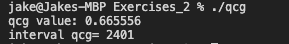
\includegraphics[width=10cm]{qcg_sc.png}
    \caption{Screenshot of output of QCG.cpp showing that interval is equal to $m$}

\end{figure}

\section*{Question 2}
Understanding the TGFSR. \\
Start off with:
$$ k =0 \rightarrow a_k = 10 $$
Bitshift $a_k$ by converting to binary and shifting 1 along
$$ a_k = 10_{10} = 1010_{2} \rightarrow 101_{2} = 5_{10} $$
Computing $(k+q) \ mod \ p$ 
$$ (k+q) \ mod \ p = (0+11) \% 25 = 11$$
The index of $(k+q) \ mod \ p$ is then 
$$ a_{(k+q) \ mod \ p} = 21 $$
Computing the first XOR :
$$ 21 \ XOR \ 5 = 16 $$
The least significant bit of $a_k$ is 0 so the second XOR is: 
$$ 16 \ XOR \ 0 = 16 $$
$$ k = k+ 1 \% 25 = 1 $$
$$ a_{k'} = 16 $$ 
Thus the new value assigned to $a_0$ is $16$. 
\begin{figure}[h]
    \centering
    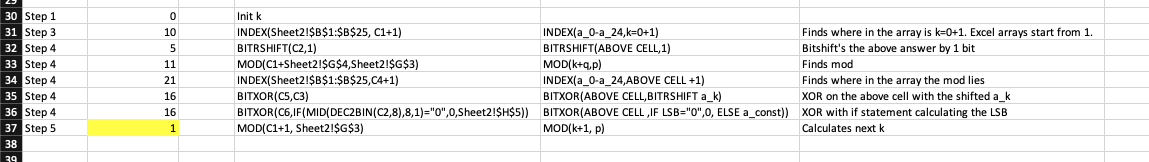
\includegraphics[width=15cm]{excel.png}
    \caption{I calculated this in excel. Here is a screenshot}

\end{figure}

\section*{Question 3}
Under the \lstinline{Chi2.cpp} program you will find a program to output the random numbers to .txt using the various array functions found in \lstinline{rng.h}. It was easier to take the arrays of random numbers and computer the $\chi^2$ value in python. \\
\\
As we can see by the uniform distirbutions. The MT and PM are more 'noisy' and less uniform whereas the LCG and QCG are fairly uniform. This is shown by the chi2 values calcuated. The MT and PM generate good $\chi^2$ values whereas the LCG and QCG do not. Unfortunately this was done for just 1 run and thus the average is not very accurate.\\



\begin{figure}[h]
    \centering
    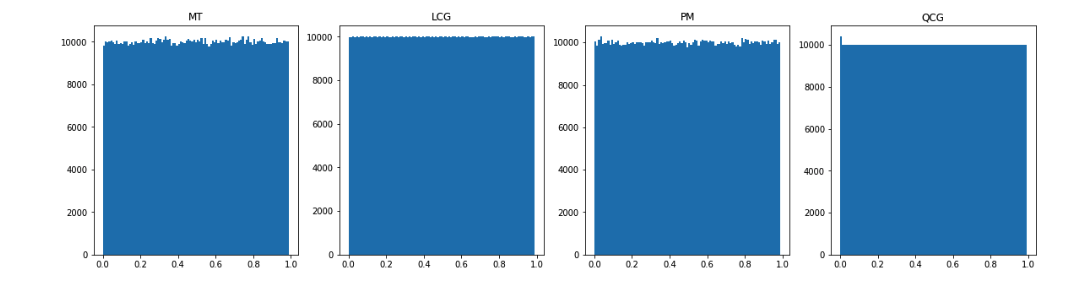
\includegraphics[width=15cm]{Uniform_dist.png}
    \caption{Uniform Distribution of the $1e6$ random numbers}

\end{figure}
\begin{figure}[h]
    \centering
    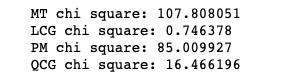
\includegraphics[width=15cm]{chi2.png}
    \caption{$\chi^2$ sum for each of the Distribution}

\end{figure}

\begin{figure}[h]
    \centering
    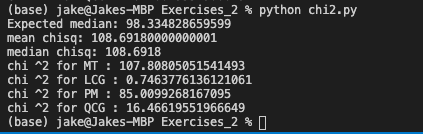
\includegraphics[width=15cm]{chisqm.png}
    \caption{$\chi^2$ sum for each of the Distribution}

\end{figure}

\section*{Question 4} 
Performing the autocorrelation test for LCG and Park-Miller Generators. This is shown in \lstinline{autocorr_test.cpp}. This file runs by specifying your output file and the number of points ($10^5$) on the run line from the command line. The program works by splitting the autocorrelation test formula into the mean, mean squared and the variance. The program then outputs the autocorrelation results along with the index number to a .dat file. The .dat file is then read in and plotted with pyplot as shown in the \lstinline{plot_q3.py} \\
\\
As you can see with the plots the LCG is not as good as it's PM counterpart. Note that I also included the inbuilt rand() function as well as the Mersenne Twister for comparison. Interestingly the LCG shuffle did not change the results for the autocorrelation. The result for the original LCG is to be expected because the values will correlate after its period. \\
\\
To calculate the LCG shuffle (implemented in rng.h) I used the Bays-Durham shuffled used in ran1 in Numerical Recipes but adapters for LCG. \\



\begin{figure}[h]
    \centering
    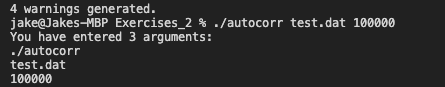
\includegraphics[width=15cm]{autocorr_1.png}
    \caption{Command Line arguments shown for autocorrelation}

\end{figure}

\begin{figure}[h]
    \centering
    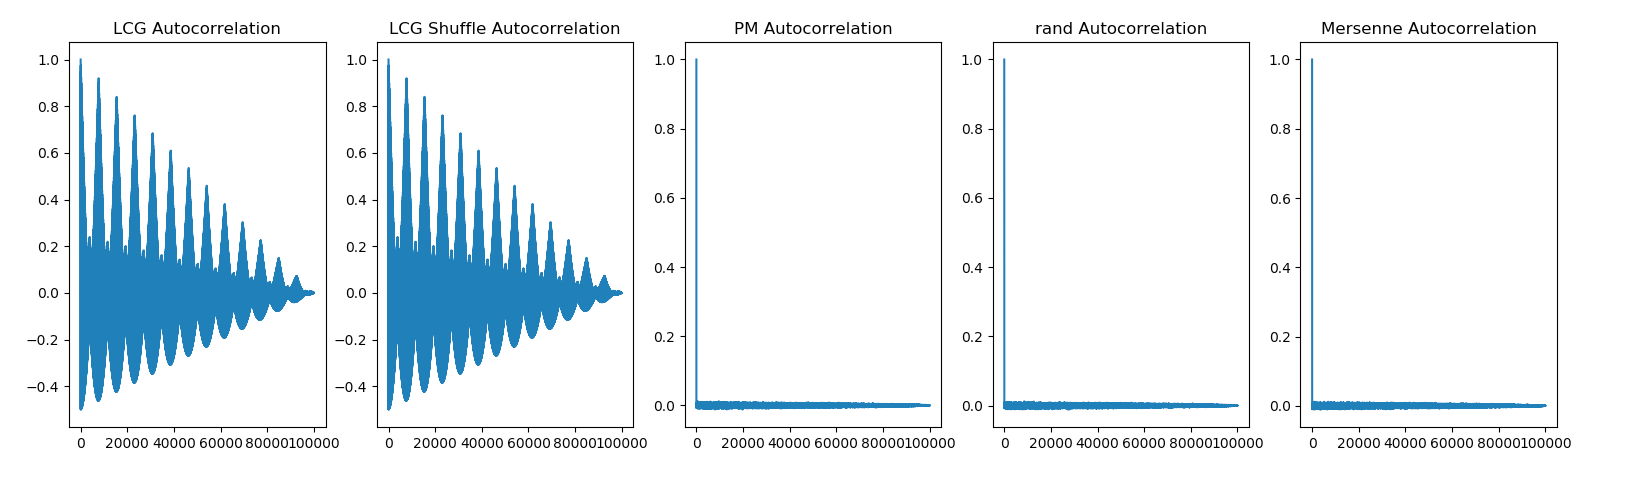
\includegraphics[width=15cm]{autocorr_2.png}
    \caption{Plot for the results of the autocorrelation}

\end{figure}



\end{document}


